%----------------------------------------------------------------------------------------

\documentclass{article}
\usepackage[czech]{babel}
\usepackage[utf8]{inputenc}
\usepackage{verbatim}
\usepackage{listingsutf8}
\usepackage{graphicx}
\usepackage{hyperref}

\hypersetup{
    colorlinks=true,
    linkcolor=blue,
    filecolor=magenta,
    urlcolor=cyan,
}

\setlength\parindent{0pt} % Removes all indentation from paragraphs

\renewcommand{\labelenumi}{\alph{enumi}.} % Make numbering in the enumerate environment by letter rather than number (e.g. section 6)
\usepackage{xcolor}
\lstset{
    language=bash, %% Troque para PHP, C, Java, etc... bash é o padrão
    basicstyle=\ttfamily\small,
    numberstyle=\footnotesize,
    numbers=left,
    backgroundcolor=\color{gray!10},
    frame=single,
    tabsize=2,
    rulecolor=\color{black!30},
    title=\lstname,
    escapeinside={\%*}{*)},
    breaklines=true,
    breakatwhitespace=true,
    framextopmargin=2pt,
    framexbottommargin=2pt,
    extendedchars=false,
    inputencoding=utf8
}

%\usepackage{times} % Uncomment to use the Times New Roman font

%----------------------------------------------------------------------------------------
%	DOCUMENT INFORMATION
%----------------------------------------------------------------------------------------

\title{Zpracování signálů} % Title

\author{Bc. Aleš Ryška} % Author name

\date{\today} % Date for the report

\begin{document}

\maketitle % Insert the title, author and date

% If you wish to include an abstract, uncomment the lines below
% \begin{abstract}
% Abstract text
% \end{abstract}

%----------------------------------------------------------------------------------------
%	SECTION 1
%----------------------------------------------------------------------------------------

\section{Zadání}
Navzorkujte napěťový signál y dle následující definice:\\
$y = 5cos(2 \pi f_1 t)-2sin(2\pi f_2 t) t\in <0,500>ms $\\
$f_s = 200 Hz, f_1 = 2Hz, f_2 = 8Hz$\\

Signál vhodně vykreslete a vypočítejte tyto charakteristiky a zobrazte je v přehledné tabulce:
\begin{itemize}
	\item střední hodnotu (mean)
	\item efektivní hodnotu (rms)
	\item rozptyl (var)
	\item směrodatnou odchylku (std)
	\item medián (median)
	\item okamžitý výkon
	\item střední výkon
	\item energii
\end{itemize}


\section{Vypracování}
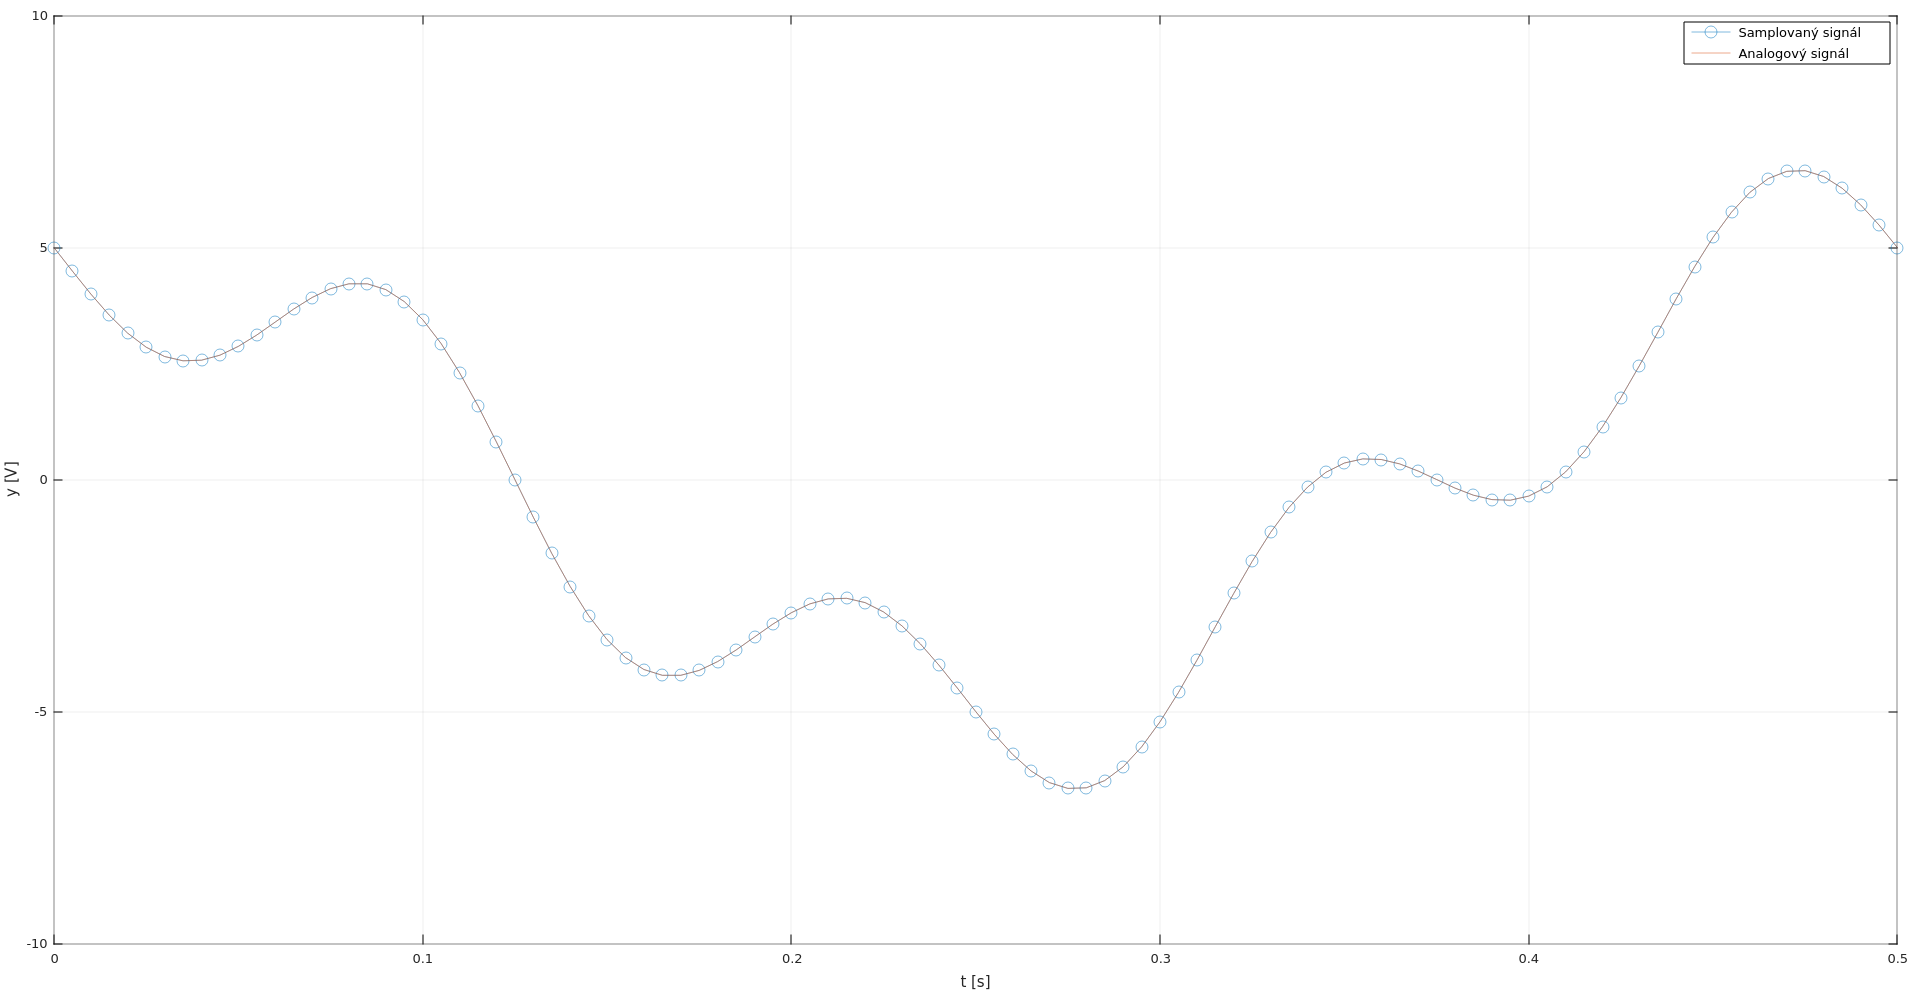
\includegraphics[scale=0.25]{../assets/img2.png}
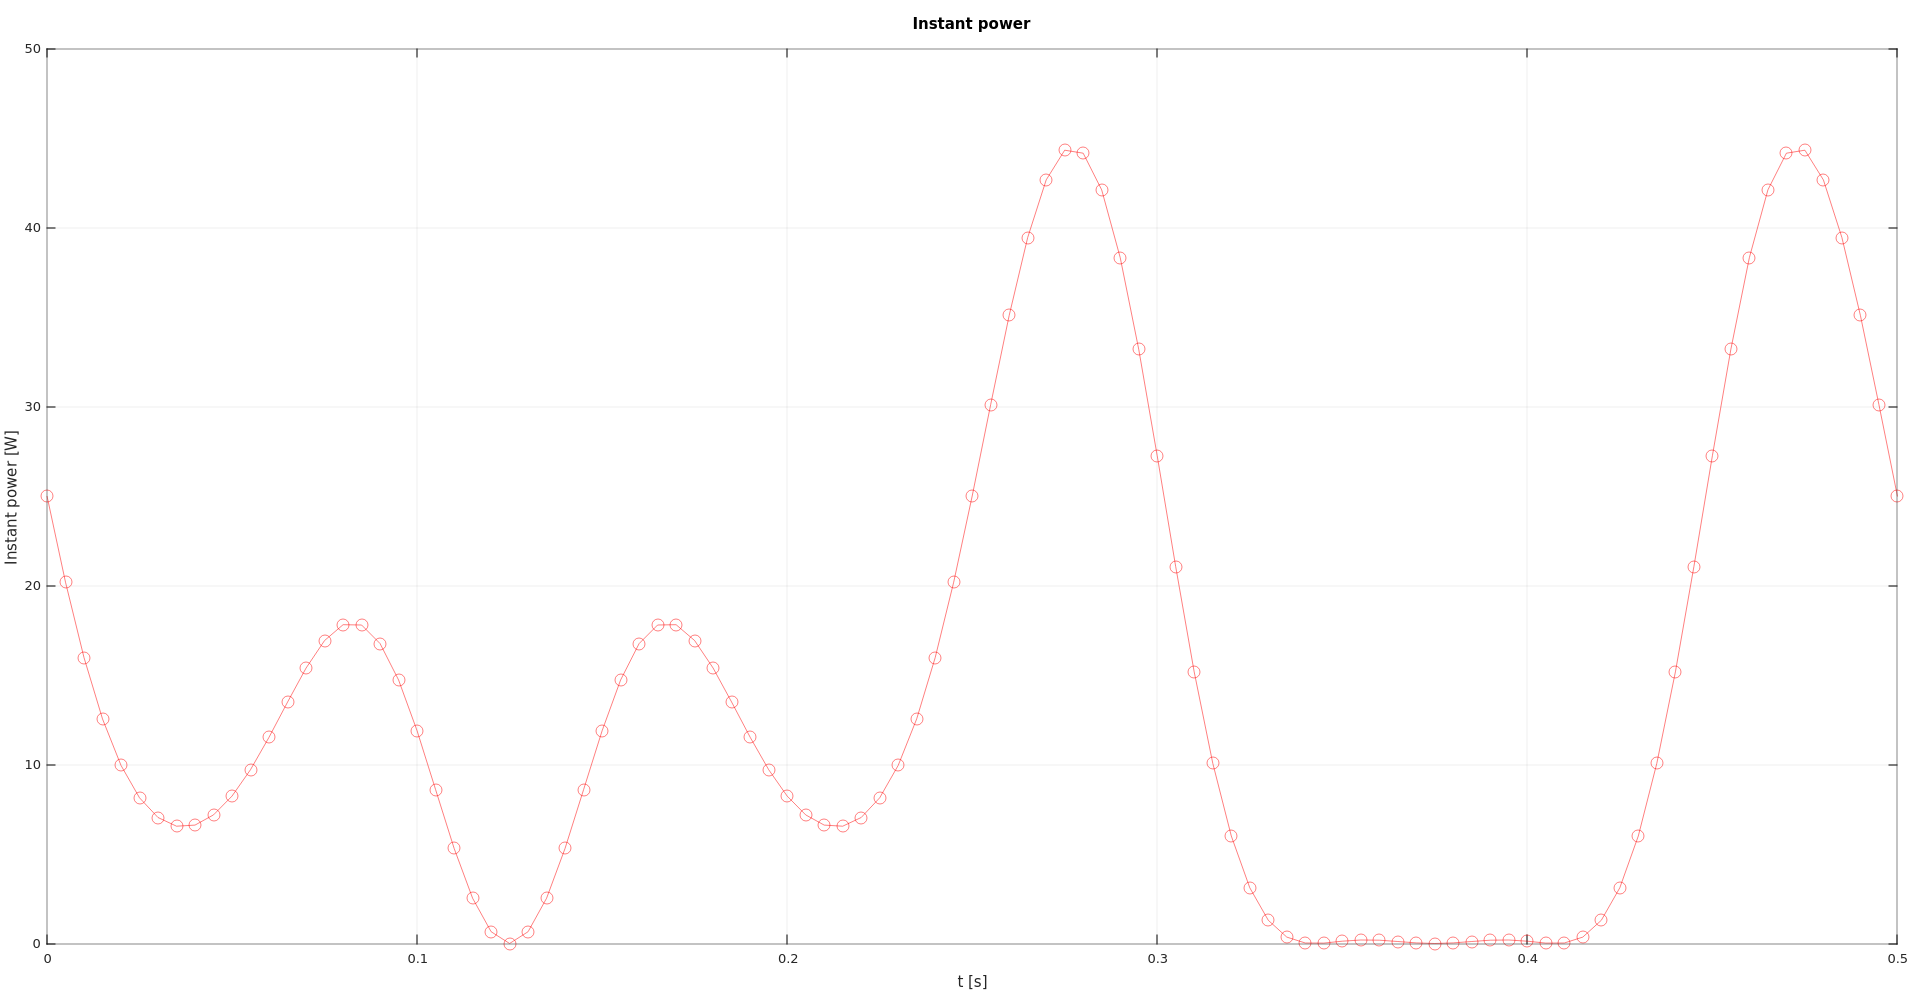
\includegraphics[scale=0.25]{../assets/img.png}
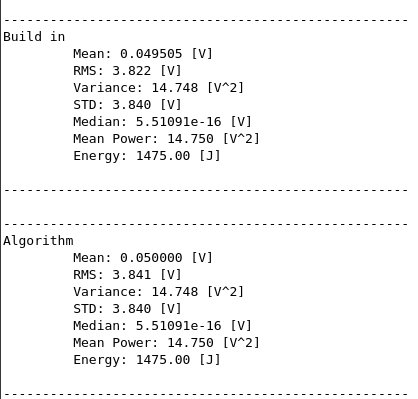
\includegraphics[scale=0.25]{../assets/img3.png}
\newpage
\section{Kód}
%--------------------------------------------------------------------------------------------------
%	CODE
%--------------------------------------------------------------------------------------------------
\lstinputlisting[language=Octave]{../code/signal_char.m}
\href{https://github.com/AleshR/AP8ZS}{Odkaz na kompetní repozitář se cvičeními}
\end{document}

